\documentclass{beamer}

\usepackage{amsmath} 

\usepackage{algpseudocode}
\usepackage{algorithm}
\algnewcommand{\LineComment}[1]{\State \(\triangleright\) #1}

\makeatletter
\renewcommand{\ALG@name}{Algoritmo}
\makeatother

\setbeamertemplate{footline}[frame number]
\beamertemplatenavigationsymbolsempty
\usecolortheme{beaver}

\newcommand{\un}[1]{\;\text{#1}}

\AtBeginSection[]
{
  \begin{frame}
    \frametitle{Sumário}
    \tableofcontents[currentsection]
  \end{frame}
}

\title[Short Paper Title]  
{Trabalho Computacional 01}

\subtitle
{Teoria da Decisão (ELE088)}

\author 
 { Raphael Henrique Braga Leivas \\
 Milton Pereira Bravo Neto \\ 
 Daniel Felipe de Almeida Araújo}


\institute 
{
Curso de Bacharelado em Engenharia de Sistemas\\
Universidade Federal de Minas Gerais
}

\date{}


\begin{document}

\begin{frame}
    \titlepage
\end{frame}

\section{Modelagem}
    
    \subsection{Problema 1 Isolado}
    \begin{frame}
        \frametitle{Problema 1 Isolado}

        \begin{center}
            Problema 1: minimização do custo de manutenção total
        \end{center}

        \vspace{0.5cm}

        \textbf{Variável de decisão:}

        \[  x_{ij}: \un{se a máquina $i$ executa a manutenção $j$}  \]
        
        \[ x_{ij} \in \{0,1\} \quad , \quad i = \{1, 2, ..., N\}  \quad , \quad j = \{1, 2, ..., J\} \]

        \vspace{0.5cm}

        \textbf{Função Objetivo e Restrições}

        \[  \min f_1 = \sum_{i=1}^{N} \sum_{j=1}^{J} c_j x_{ij} \]

        \[ \sum_{j=1}^{J} x_{ij} = 1 \quad , \quad \forall i = {1, 2, ..., N} \]
    \end{frame}

    \begin{frame}
        \frametitle{Problema 1 Isolado - Solução Trivial}

        \begin{center}
            Atribuir a manutenção mais barata a todos os equipamentos:
        \end{center}


        \[ x^{*} = \begin{bmatrix} 
            1 & 0 & 0 \\
            1 & 0 & 0 \\
            \vdots & \vdots & \vdots \\
            1 &  0      & 0 
            \end{bmatrix} \]

        \vspace{1cm}

       \[ f_1\left(x^{*}\right) =  0 \]
    \end{frame}

    \subsection{Problema 2 Isolado}
    \begin{frame}
        \frametitle{Problema 2 Isolado}

        \begin{center}
            Problema 2: minimização do custo esperado de falha total
        \end{center}

        \vspace{0.5cm}

        \textbf{Variável de decisão:}

        \[  x_{ij}: \un{se a máquina $i$ executa a manutenção $j$}  \]
        
        \[ x_{ij} \in \{0,1\} \quad , \quad i = \{1, 2, ..., N\}  \quad , \quad j = \{1, 2, ..., J\} \]

    \end{frame}

    \begin{frame}
        \frametitle{Problema 2 Isolado}

        \textbf{Função Objetivo}

        \[  \min f_2 = \sum_{i=1}^{N} \sum_{j=1}^{J} p_{ij} \, d_i \, x_{ij} \]

        \[ x_{ij} \in \{0,1\} \quad , \quad i = \{1, 2, ..., N\}  \quad , \quad j = \{1, 2, ..., J\} \]

        \[ 
        p_{ij} = \frac{F_i \left(t_0 + k_j \Delta t \right) - F_i\left(t_0\right) }{1 - F_i\left(t_0\right)}
        \quad , \quad 
        F_i(t) = 1 - \exp \left[ - \left( \frac{t}{\eta_i} \right)^{\beta_i} \right] 
        \]

        \vspace{0.5cm}
        
        \textbf{Restrição}

        \[ \sum_{j=1}^{J} x_{ij} = 1 \quad , \quad \forall i = {1, 2, ..., N} \]
    \end{frame}

    \begin{frame}
        \frametitle{Problema 2 Isolado - Solução via Simplex}

        \begin{center}
            Atribuir a manutenção mais cara a todos os equipamentos:
        \end{center}

        \[ x^{*} = \begin{bmatrix} 
            0 & 0 & 1 \\
            0 & 0 & 1 \\
            \vdots & \vdots & \vdots \\
            0 &  0      & 1 
            \end{bmatrix} \]

        \vspace{1cm}

       \[ f_2\left(x^{*}\right) = 1048.17 \]
    \end{frame}

\section{Algoritmos}

\subsection{Representação Computacional}
    \begin{frame}
        \frametitle{Representação Computacional}

        \begin{itemize}
            \item Vetor de tamanho $N = 500$
            \item Cada posição $i$ indica o custo da manutenção associada ao equipamento $i$
        \end{itemize}

        \[ x = \begin{bmatrix} 2 & 0 & 1 & \cdots & 2 \end{bmatrix} \]

        \begin{itemize}
            \item Equipamento 1 executa manuteção de custo 2
            \item Equipamento 2 executa manuteção de custo 0
            \[  \cdots  \]
            \item Equipamento 500 executa manuteção de custo 2
        \end{itemize}
    \end{frame}


\subsection{BVNS - Basic Variable Neighborhood Search}
    \begin{frame}
        \frametitle{BVNS - Basic Variable Neighborhood Search}
        \begin{algorithm}[H]
            \caption{BVNS implementado no trabalho.}\label{alg:bvns}
            \begin{algorithmic}[1]
            \Procedure{BVNS}{\textbf{x}, k\textsubscript{max}}
                \While{num\_sol\_avaliadas $<$ max\_sol\_avaliadas}
                    \State k $\gets$ 1
        
                    \While{k $<$ k\textsubscript{max}}
                        \State $ \textbf{x'} \gets$ \Call{Shake}{\textbf{x}, k} 
                        \State $ \textbf{x''} \gets$ \Call{FirstImprovement}{\textbf{x}, \textbf{x'}, k} 
                        \State $ \textbf{x}, k \gets$ \Call{NeighborhoodChange}{\textbf{x}, \textbf{x''}, k} 
                    \EndWhile
                \EndWhile
            \EndProcedure 
            \end{algorithmic}
        \end{algorithm}
    \end{frame}

    \begin{frame}
        \frametitle{BVNS - Basic Variable Neighborhood Search}
        \begin{algorithm}[H]
            \caption{Função Shake.}\label{alg:shake}
            \Comment{Gera uma solução aleatória na k-ésima estrutura de vizinhança.}
            \begin{algorithmic}[1]
            \Procedure{Shake}{\textbf{x}, k}
                \If{k = 1}
                    \State $\textbf{y} \gets$ 1-swap
                \EndIf
                \If{k = 2}
                    \State $\textbf{y} \gets$ Troca de planos de manutenção entre dois equipamentos
                \EndIf
                \If{k = 3}
                    \State $\textbf{y} \gets$ Mudança de um bloco de 50 equipamentos para outro plano
                \EndIf
            \Statex
            \State \textbf{return y} 

            \EndProcedure 
            \end{algorithmic}
        \end{algorithm}
    \end{frame}

    \begin{frame}
        \frametitle{BVNS - Basic Variable Neighborhood Search}
        \begin{algorithm}[H]
            \caption{Função FirstImprovement.}\label{alg:first-improvement}
            \Comment{Busca uma solução na vizinhança de \textbf{x} melhor que \textbf{x}.}

            \begin{algorithmic}[1]
            \Procedure{FirstImprovement}{\textbf{x}, \textbf{x'}, k}

            \State $\textbf{N} \gets$ 100 vizinhos aleatórios da k-ésima vizinhança


            \ForAll {\textbf{v} \textbf{in} \textbf{N}}
                \If{$f(\textbf{v}) < f(\textbf{x})$}
                    \State \textbf{return v} 
                \EndIf
            \EndFor
               
            \Statex
            \State \textbf{return x} 
            \EndProcedure 
            \end{algorithmic}
        \end{algorithm}
    \end{frame}

    \begin{frame}
        \frametitle{BVNS - Basic Variable Neighborhood Search}
        \begin{algorithm}[H]
            \caption{Heurística construtiva para gerar a solução inicial.}\label{alg:sol-inicial}
            \begin{algorithmic}[1]
            \Procedure{SolucaoInicial}{\null}

            \State \textbf{x} $\gets$ Solução aleatória

            \ForAll {i \textbf{in} \textbf{x}}
                \If{variancia($p_{ij}d_{i}$) $\geq$ limiar}
                    \State \textbf{x}[i] $\gets$ Manutenção mais cara
                \Else
                    \State \textbf{x}[i] $\gets$ Manutenção mais barata
                \EndIf
            \EndFor
               
            \Statex
            \State \textbf{return x} 
            \EndProcedure 
            \end{algorithmic}
        \end{algorithm}
    \end{frame}

\section{Resultados}

\subsection{Problema 1 Isolado}
    \begin{frame}
        \frametitle{Problema 1 Isolado}

        \centering
        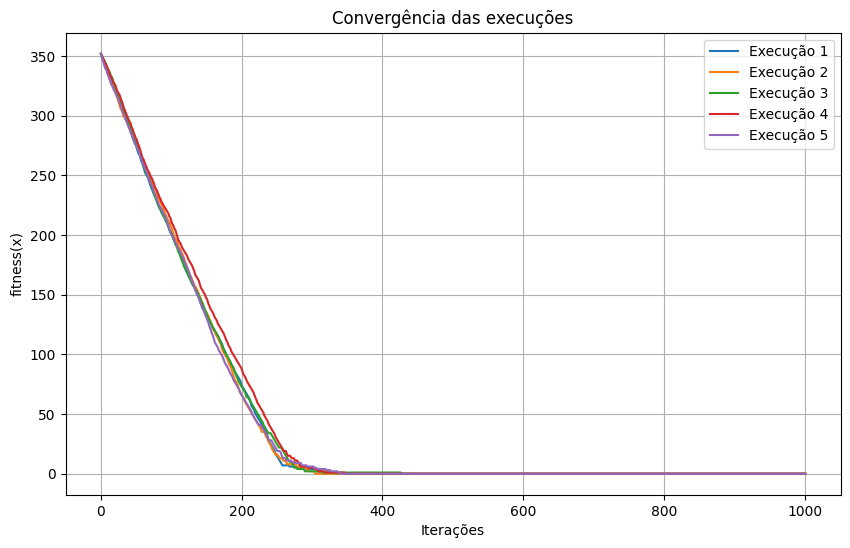
\includegraphics[width=\textwidth,trim=1 1 1 1,clip]{images/convergencia_execucoes_p1.png}
        \[  x^* = \begin{bmatrix} 0 & 0 & 0 & \cdots & 0 \end{bmatrix} \quad , \quad f\left(x^*\right) = 0 \pm 0 \]
    \end{frame}

    \subsection{Problema 2 Isolado}
    \begin{frame}
        \frametitle{Problema 2 Isolado}

        \centering
        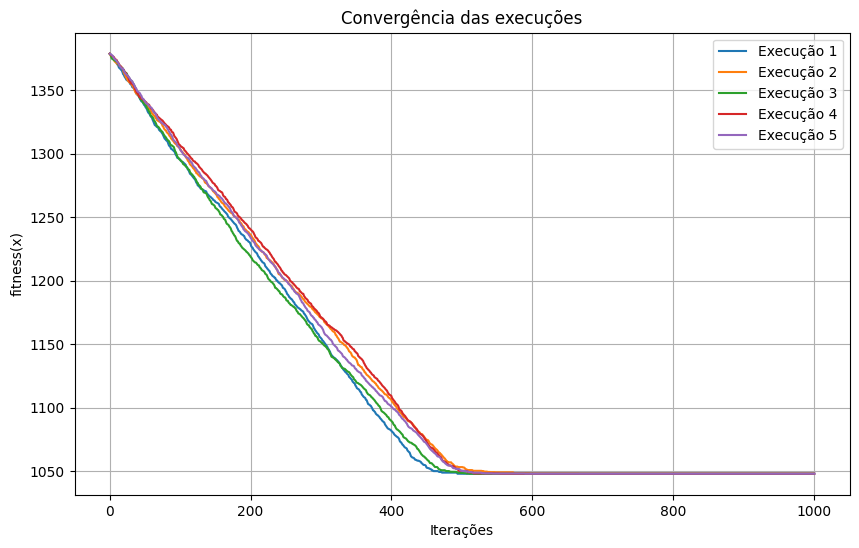
\includegraphics[width=\textwidth,trim=1 1 1 1,clip]{images/convergencia_execucoes.png}
        \[  x^* = \begin{bmatrix} 2 & 2 & 2 & \cdots & 2 \end{bmatrix} \quad , \quad f\left(x^*\right) = 1048.2 \pm 0 \]
    \end{frame}


\section{Referências}

    \begin{frame}
        \frametitle{Referências}

        \begin{itemize}
            \item M. Gendreau, J.-Y. Potvin (eds.), Handbook of Metaheuristics, Springer, 2nd ed.,
            2010.
        \end{itemize}
    \end{frame}

\end{document}